\documentclass[12pt]{jarticle}
\usepackage[dvipdfmx]{graphicx}
\usepackage[dvipdfmx]{color}
\usepackage{iepaper}

\usepackage{ccaption}
\usepackage{colortbl}
\usepackage{multirow}
\usepackage{url}
\usepackage{bm,amsmath}
\usepackage{arydshln}
\usepackage{algorithm}
\usepackage{algorithmicx}
\usepackage[noend]{algpseudocode}
\usepackage{subfigure}
\usepackage{comment}
\usepackage{txfonts}
\usepackage{inputenc}

\title{TDGA を導入した DARTS による深層学習の構造探索}
\author{杉山 竜弥}
\gakuseki{1171201092}[B] %[B]: Bachelor, [M]: Master
\group{第 1 研究グループ}
\shidou{森直樹 教授}
% \syusa{Foo Bar 教授}
% \hukusa{Hoge Hoge 教授}{Foo Foo 教授}{Bar Bar 准教授}

%図番号を「(section番号).(図番号)」とするため.
\makeatletter
\renewcommand{\thefigure}{%
	\thesection.\arabic{figure}}
\@addtoreset{figure}{section}
\makeatother
\makeatletter
\renewcommand{\thetable}{%
	\thesection.\arabic{table}}
\@addtoreset{table}{section}
\makeatother
\makeatletter
\renewcommand{\theequation}{%
	\thesection.\arabic{equation}}
\@addtoreset{equation}{section}
\makeatother

%目次・図一覧・表一覧
\begin{document}
\maketitle
\pagenumbering{roman}
\tableofcontents\newpage
\listoffigures
\newpage
\listoftables
\newpage
\pagenumbering{arabic}


%文書開始
\newpage
\changeindent{0cm}
\section{はじめに}
\label{sec:intro}
\changeindent{2cm}

機械学習の分野では, 深層学習モデルの改良によって大きく精度が向上してきた.
しかしモデルの設計とその性能の関係はブラックボックスであり
手作業によるチューニングには膨大な労力を要する.

ネットワークの探索を自動化する手法として提案された
Neural Architecture Search(NAS)はネットワークを機械学習によって探索する.
しかし何千ものGPUを必要とするため, NASに代わり小規模な資源で計算できる
Differentiable Architecture Search(DARTS) が大きな注目を集めている.
DARTSはネットワークの構造と演算子の候補を探索するが,
一方でDARTSにはネットワーク構造にいくつかの拘束条件がある.

またネットワークの構造を組み合わせ最適化と考えることもでき,
導入する手法として今回は遺伝的アルゴリズム (Genetic Algorithm: GA) に着目する.
GAは生物の進化の仕組みを模倣した最適化手法であるが,
初期段階で個体群が同じ個体で占められる初期収束問題がある.
一方Thermodynamical Genetic Algorithm (TDGA)では,
GAの選択ルールに多様性を考慮した適応度を導入することでこの初期収束問題を防ぐことができる.


本研究では演算子の種類ではなくネットワークの構造にのみ着目し,
DARTSの構造制限をなくしネットワークの柔軟な探索を目的とする.
ベースとなるネットワークを19層構造のVGG19とし,
ショートカット位置についてDARTSで探索を行う方法と, それにTDGAを導入する方法を提案する.


以下に本論文の構成を示す.まず,\ref{sec:tech} 章では本研究で用いる要素技術について概説する.
\ref{sec:pred} 章で深層学習の構造の設定と探索手法を提案する.
そして\ref{sec:exp} 章において,数値実験により手法の性能を検証し, 本研究で提案する手法の考察をする.
\ref{sec:conclusion} 章で本研究の成果をまとめたうえで,今後の課題について述べる.


\begin{comment}
\end{comment}
 %はじめに
\clearpage
\newpage
\changeindent{0cm}
\section{要素技術}
\label{sec:tech}
\changeindent{2cm}

%9-12
本章では,本研究の提案手法に用いた技術について説明する.

%LSTM
\changeindent{0cm}
\subsection{深層学習}
\changeindent{2cm}
\label{sec:02_deep}



\changeindent{0cm}
\subsection{Neural Architecture Search}
\changeindent{2cm}
\label{sec:02_nas}
Neural Architecture Search(NAS)\cite{DBLP:journals/corr/ZophL16}は,
機械学習の分野で使用されているニューラルネットワークの設計を自動化する手法である.
ニューラルネットワークの設計は直感的でなく,
チューニングに人による労力を多く必要とするため,
ニューラルネットワークの設計は非常に困難である.

NASはニューラルネットワークが構造に関する設定の文字列で表現できることを利用して,
この文字列を生成する
Recurrent Neural Network(RNN)を
強化学習 Reinforcement Learning(RL)によって学習する.



\changeindent{0cm}
\subsection{Differentiable Architecture Search}
\changeindent{2cm}
\label{sec:02_darts}

Differentiable Architecture Search(DARTS)\cite{DBLP:journals/corr/abs-1806-09055}は,
離散的なアーキテクチャ探索空間に強化学習を適用したNASとは異なり,
微分可能な方法で定式化し,
偏微分による勾配降下法を使用してアーキテクチャを効率的に探索する手法である.

探索空間を連続にするため, カテゴリカルな演算子の選択の代わりに, 候補全ての可能性をもつ混合演算子を
(\ref{eq:darts/operation}) 式で定義する.
アーキテクチャを有向非巡回グラフで表したとき, ノードを潜在的な特徴表現 $x^{(i)}$,
エッジを特徴 $x^{(i)}$ が適用される関数 $o(・)$ とすると,
\begin{equation}
  \label{eq:darts/operation}
  \bar{o}^{(i, j)}(x) = \sum_{o \in \mathcal{O}} \frac{\exp(\alpha^{(i, j)}_o)}{\sum_{o' \in \mathcal{O}} \exp(\alpha^{(i, j)}_{o'})} o(x)
\end{equation}
となる. ここで
$\mathcal{O}$ は探索する演算子の候補集合,
$\alpha^{(i, j)}$ はエッジ $(i, j)$ の混合演算子の重みベクトルである.
DARTSは勾配降下法によって連続変数集合$\alpha$を学習する.

$\alpha$ とレイヤーの重み $w$ のBi-Level最適化問題を $w$ の近似によって同時に学習し,
NASにおいて 3000 GPU days 必要なタスクに対してDARTSは 3.3 GPU days まで高速化した.

DARTSでは次元を統一するためセルと呼ぶ小さなネットワーク構造を重ねたモデルを利用する.
セルを構成するノードは2つのノードからの演算子エッジを持ち,
どのノードからの演算子を選ぶのかをアーキテクチャを示す重み $\alpha$ によって決定する.
DARTSの問題点として位置と演算子の種類は探索できるが,
大局的な構造やノードの持つエッジ数など固定されたアーキテクチャにしか適用できない点が挙げられる.


\changeindent{0cm}
\subsection{Genetic Algorithm}
\changeindent{2cm}
\label{sec:02_ga}
遺伝的アルゴリズム(Genetic Algorithm : GA)は生物の進化の仕組みを模倣した最適化手法である.
問題の解候補を遺伝子の持つ個体として表現し, 適応度によって個体を評価・選択する.
交叉・突然変異などの操作によって解候補の多様性を保ちつつ,
近傍を探索しながら世代を重ねて近似的な最適解を求める.
% GAに必要な条件は評価関数の全順序性と探索空間が位相を持つことである.

% 整数値と実数値

% 初期収束問題
GAには偶然適応度の高くなった個体だけが選択され続け,
個体群を同じ個体が占める初期収束問題がある.
問題によって適切な交叉・突然変異を設定する必要がある.


\changeindent{0cm}
\subsection{Thermo?? Dinamic?? Genetic Algorithm}
\changeindent{2cm}
\label{sec:02_tdga}


% \begin{eqnarray}
% s_{t} &=& f(U_{x_{t}}+W_{s_{t-1}}) \nonumber \\
% y_{t} &=& g(V_{s_{t}}) \nonumber \\[8pt]
% f(z) &=& \frac{1}{1+\exp(-z)} \nonumber \\[8pt]
% g(z_{m}) &=& \frac{\exp(z_{m})}{\sum_{k}\exp(z_{k})} \nonumber
% \end{eqnarray}
%
% \begin{figure}[t]
%      \begin{center}
%        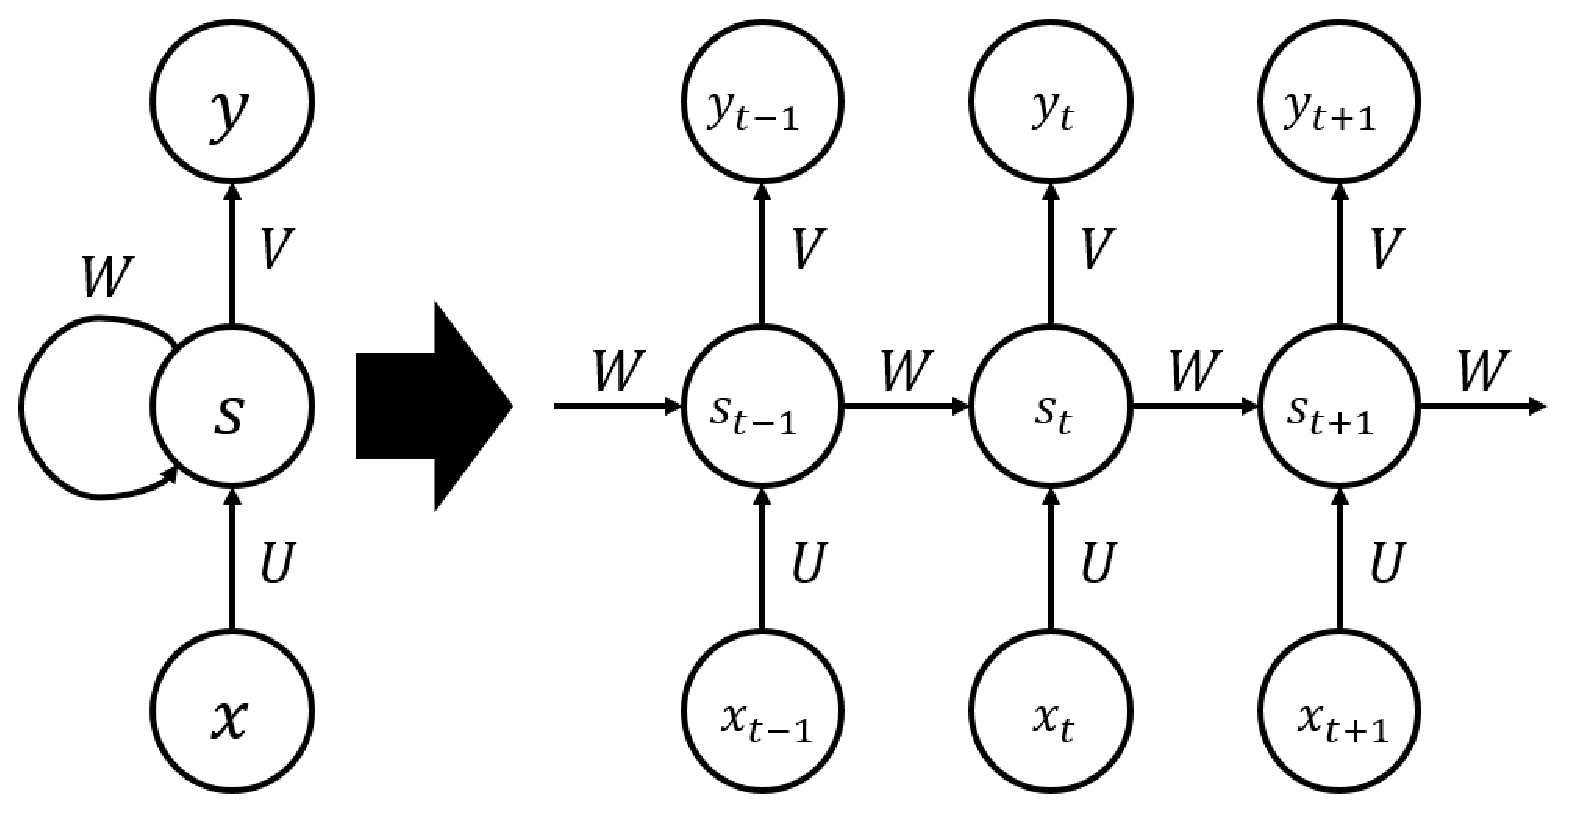
\includegraphics[width=12cm,clip]{./fig/02.tech/rnn.eps}
%       \end{center}
%       \caption{RNN ネットワーク}
%      \label{fig:02_net}
% \end{figure}
 %要素技術
\clearpage
\newpage
\changeindent{0cm}
\section{ショートカット探索}
\label{sec:pred}
\changeindent{2cm}

\begin{figure}[t]
  \begin{center}
    \includegraphics[clip,width=6cm]{./fig/03.pred/image.png}
  \end{center}
  \caption{ショートカット概念図}
  \label{fig:image}
\end{figure}

DARTS で柔軟なアーキテクチャを探索することを実験の目的とし, 構造探索タスクとして
深層畳み込みネットワークの VGG19\cite{Simonyan15} の
ショートカット接続\cite{mao2016image}を考える.
図 \ref{fig:image} のように, ショートカット接続は,
畳み込み部において 1 つ以上特徴を飛ばした接続とする.
VGG19 は分岐がない単純なネットワーク構造であるため, ベースモデルに適しているとして選択した.

VGG19 は 16 層の畳み込み層と 3 層の線形結合層を持つ.
表 \ref{tab:vgg} は, VGG19 の畳み込みニューラルネットワーク
(Convolutional Neural Network: CNN) 部分の構造を示している.
構成する関数は, フィルターサイズが 3 $\times$ 3 の畳み込み層 (Conv2d) ,
Batch Normalization (BN)\cite{Ioffe2015BatchNA} ,
活性化関数 (Rectified Linear Unit: ReLU) ,
ストライドが 2 の Max Pooling (MaxPool) である.
この VGG19 に対し層を飛ばして接続するショートカットの数と位置を求め,
性能を向上させることを目的とする.

\begin{table}[t]
  \begin{center}
    \caption{VGG19 の構造}
		\vspace{-1mm}
    例として入力する画像を (32, 32, 3) 次元としている.
		\vspace{1mm}
		\vspace{3mm}
    \begin{tabular}{|c|c|c|l|}
    \hline
    \textbf{index} & \textbf{image size} & \textbf{channels} & \multicolumn{1}{c|}{\textbf{applied function}} \\ \hline
    input & 32 $\times$ 32 & 3   & \multicolumn{1}{c|}{-}         \\ \hline
    1     & 32 $\times$ 32 & 64  & 3$\times$3\_Conv2d, BN, ReLU          \\ \hline
    2     & 16 $\times$ 16 & 64  & 3$\times$3\_Conv2d, BN, ReLU, MaxPool \\ \hline
    3     & 16 $\times$ 16 & 128 & 3$\times$3\_Conv2d, BN, ReLU          \\ \hline
    4     & 8 $\times$ 8   & 128 & 3$\times$3\_Conv2d, BN, ReLU, MaxPool \\ \hline
    5     & 8 $\times$ 8   & 256 & 3$\times$3\_Conv2d, BN, ReLU          \\ \hline
    6     & 8 $\times$ 8   & 256 & 3$\times$3\_Conv2d, BN, ReLU          \\ \hline
    7     & 8 $\times$ 8   & 256 & 3$\times$3\_Conv2d, BN, ReLU          \\ \hline
    8     & 4 $\times$ 4   & 256 & 3$\times$3\_Conv2d, BN, ReLU, MaxPool \\ \hline
    9     & 4 $\times$ 4   & 512 & 3$\times$3\_Conv2d, BN, ReLU          \\ \hline
    10    & 4 $\times$ 4   & 512 & 3$\times$3\_Conv2d, BN, ReLU          \\ \hline
    11    & 4 $\times$ 4   & 512 & 3$\times$3\_Conv2d, BN, ReLU          \\ \hline
    12    & 2 $\times$ 2   & 512 & 3$\times$3\_Conv2d, BN, ReLU, MaxPool \\ \hline
    13    & 2 $\times$ 2   & 512 & 3$\times$3\_Conv2d, BN, ReLU          \\ \hline
    14    & 2 $\times$ 2   & 512 & 3$\times$3\_Conv2d, BN, ReLU          \\ \hline
    15    & 2 $\times$ 2   & 512 & 3$\times$3\_Conv2d, BN, ReLU          \\ \hline
    16    & 1 $\times$ 1   & 512 & 3$\times$3\_Conv2d, BN, ReLU, MaxPool \\ \hline
    \end{tabular}
    \label{tab:vgg}
  \end{center}
\end{table}


モデル中の潜在的特徴は高さ・幅・チャンネル数を持つデータであるが,
特徴の次元は場所によって異なるため, ショートカットは次元を変換する必要がある.
したがってショートカット関数は以下のように設定した.
\begin{enumerate}
  \item 次元が同じ場合:恒等関数
  \item チャンネル数が違う場合:Pointwise Convolution
  \item 高さと幅が半分の場合:Factorized Reduce
  \item それ以外の場合:ショートカットを定義しない
\end{enumerate}
Pointwise Convolution は, 要素ごとの畳み込みでチャンネル数を調整する.
Factorized Reduce は, 畳み込み層を偶数列と奇数列の 2 枚 用いることで, 情報の損失を防ぎつつ特徴次元を半分にすることができる.

ショートカットに使用する関数の制限によってショートカット位置の候補は 61 であるため,
探索空間は $2^{61}$ である.
演算子の種類は固定することで, アーキテクチャ $\bm{\alpha}$ は畳み込み部に相当するグラフの重みをもつ隣接行列と定義した.


%4.1
\changeindent{0cm}
\subsection{提案手法 : DARTS}
\label{sec:pred.01}
\changeindent{2cm}

DARTS でネットワーク構造を探索するときの, 学習の手順は
\begin{enumerate}
  \item 探索:アーキテクチャ $\bm{\alpha}$ の訓練
  \item 構成:$\bm{\alpha}$ からネットワークを構成
  \item 評価:得られたネットワークをバックプロパゲーションにより訓練し, テストデータで性能を評価
\end{enumerate}
の 3 段階から成る.


\subsubsection{探索}

探索段階では, 勾配降下法によって $\bm{\alpha}$ の更新を行う.
このとき探索用のネットワークは, ショートカットの本数も探索するため,
$\bm{\alpha}$ に対する重み補正 $\bm{\beta}$ を用いて (\ref{equ:cut}) 式 で定義する.

\begin{equation}
  \label{equ:cut}
  \bm{x}_i = f^{\mathrm{c}}_{i-1, i}(\bm{x}_{i-1}) + \bm{\beta}_i \sum_{j \in S_i} \bm{\alpha}_{ij} f^{\mathrm{s}}_{j, i} (\bm{x}_j)
\end{equation}

ここで $f^{\mathrm{c}}(・)$, $f^{\mathrm{s}}(・)$ は, VGG の畳み込み関数とショートカット関数,
$S_i$ はノード $i$ とショートカットで接続する先行 (predecessor) ノードのインデックス集合である.

ただし $\bm{\beta}=0$ で勾配の更新ができなくなるので,
\begin{equation}
  \label{equ:beta}
  \hat{\bm{\beta}} = \begin{cases}
    \exp(\bm{\beta} - 1) & (\bm{\beta} \leq 1) \\
    \log(\bm{\beta}) + 1 & (\mathrm{otherwise})
  \end{cases}
\end{equation}
で 0 とならないように補正した $\hat{\bm{\beta}}$ を用いた.

\begin{figure}[t]
  \begin{center}
    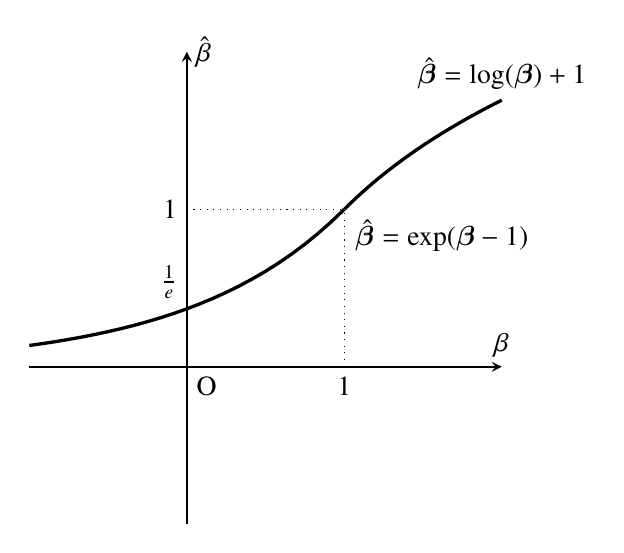
\begin{tikzpicture}
      \begin{scope}[scale=2]
        \draw[->,>=stealth,semithick] (-1,0)--(2,0)node[above]{$\beta$}; %x軸
        \draw[->,>=stealth,semithick] (0,-1)--(0,2)node[right]{$\hat{\beta}$}; %y軸
        \draw(0,0)node[below right]{O}; %原点
        \draw(1,0)node[below]{$1$}; %点(-1,0)
        \draw(0,1)node[left]{$1$}; %点(0,1)
        \draw(0,{1/e})node[above left]{$\frac{1}{e}$}; %点(0,1)
        \draw[dotted,domain=0:1] plot(\x,{1});
        \draw[dotted,domain=0:1] plot({1}, \x);
        \draw[very thick, domain=1:2] plot(\x,{ln(\x)+1})node[above]{$\hat{\bm{\beta}} = \log(\bm{\beta}) + 1$};
        \draw[very thick, domain=-1:1] plot(\x,{exp(\x - 1)})node[below right]{$\hat{\bm{\beta}} = \exp(\bm{\beta} - 1)$};
      \end{scope}
    \end{tikzpicture}
  \end{center}
  \caption{$\bm{\beta}$ の補正関数}
  \label{fig:pred/beta}
\end{figure}




\subsubsection{構成}

構成段階では, 探索段階で得られた $\bm{\alpha}$ から具体的なネットワークをサンプリングする.
$\bm{\alpha}$ の値に対する, ネットワークの構成手法はいくつか考えられるため,
\begin{itemize}
  \item 構成手法 A : predecessors の中で大きい順に採択
  \item 構成手法 B : 閾値以上のエッジを採択
\end{itemize}
の 2 通りの手法を設定した.
% (predecessorsはあるノードに接続している前のノードの集合)

\subsubsection{評価}
評価段階では, 構成段階で得られたネットワークを学習し,
最大の正答率をネットワークの性能とする.
このときのパラメータは, グリッドサーチによる最適化 API の Optuna \cite{akiba2019optuna}
で事前学習した結果から設定する.




\clearpage\newpage
\changeindent{0cm}
\subsection{提案手法 : DARTS + TDGA}
\label{sec:pred.02}
\changeindent{2cm}

\begin{figure}[t]
  \begin{center}
    \includegraphics[clip,width=6cm]{./fig/03.pred/datdga.png}
  \end{center}
  \caption{提案手法 : DARTS + TDGA 概念図}
  \label{fig:image_ga}
\end{figure}

実験 1 では $\bm{\alpha}$ の学習程度によって重み $\bm{w}$ の学習しやすさに偏りがあったため,
収束するグラフ構造にばらつきが見られた.

そこで実験 1 から得られた構造探索のための実験設定をもとに,
個体表現を $\bm{\alpha}$ とした遺伝的アルゴリズムによって,
アーキテクチャを複数同時に管理, 最適化し,
個体群の多様性を維持しつつ, 安定的なネットワーク構造の学習を図った.
単純に個体数を増やすと計算コストが定数倍されるため,
重み $\bm{w}$ は全体で共有する One-Shot モデルを利用することで高速化した.


\subsubsection{多様性項の拡張}
(\ref{eq:Entropy}) 式では, 多様性の計算にエントロピーを利用していたが,
個体 $\bm{\alpha}$ は実数値の行列であるためエントロピーは計算できない.

\begin{equation}
H = \sum_{k \in \mathcal{P}} \sqrt{\mathrm{MSE}(\bm{\alpha}_k, \bar{\bm{\alpha}})} \label{eq:Entropy-new}
\end{equation}

そこで行列の各要素の標準偏差の平均として, $H$ の実数値拡張をした.


\subsubsection{実験手順}
実験は 3 段階からなり, 事前学習した DARTS から, $\bm{w}$, $\bm{\alpha}$ を引き継ぎ,
TDGA で再探索し, 得られた最良個体のアーキテクチャを学習して性能を評価する.
図 \ref{fig:image_ga} に $\bm{w}$, $\bm{\alpha}$ の関係を示す.

\begin{enumerate}
  \item 事前学習
  \item アーキテクチャ再探索
  \item 性能評価
\end{enumerate}

\subsubsection{事前学習}

事前学習では, TDGA に引き継ぐための初期値を DARTS で学習する.
実験 1 の結果から辺ごとに計算する手法が有効であるとわかったため,
正規化として先行研究の DARTS でも利用されていた,
Softmax ではなく Hard Sigmoid に変更する.
この変更によって, $\alpha$ の正規化された値と生の値の相互変換ができるようになり,
実験間のデータ受け渡しが容易となった.


\subsubsection{アーキテクチャ再探索}

以下に TDGA をベースとして, DARTS の学習ステップの追加と多様性項の実数値拡張をした提案手法のアルゴリズム

\begin{itemize}
  \item 提案手法 1. DARTS + TDGA ($\bm{w}$, $\bm{\alpha}$)
  \item 提案手法 2. DARTS + TDGA ($\bm{\alpha}$)
  \item 提案手法 3. DARTS + TDGA
\end{itemize}

\noindent
を アルゴリズム \ref{alg1}, \ref{alg2}, \ref{alg3} に示す.
アルゴリズム \ref{alg1} をベースとして, DARTS による勾配更新のステップを無効にすることで,
DARTS が TDGA の学習に与える影響をみる.

\begin{algorithm}[tb]
  \caption{提案手法 1. DARTS + TDGA ($\bm{w}$, $\bm{\alpha}$)}
  \label{alg1}
  \begin{enumerate}
    \item DARTSで事前学習したモデルの重みを引き継いだ初期個体を生成
    \item 重み $\bm{w}$ を $\displaystyle \nabla_{\bm{\alpha}} \mathcal{L}_{\mathrm{train}}(\bm{w}, \bar{\bm{\alpha}})$ で更新
    \item 個体 $\bm{\alpha}_i$ を $\displaystyle \nabla_{\bm{\alpha}} \mathcal{L}_{\mathrm{valid}}(\bm{w}, \bm{\alpha}_i)$ で更新
    \item 適応度 $\displaystyle \mathcal{L}_{\mathrm{test}}(\bm{w}, \bm{\alpha}_i)$ で個体 $\bm{\alpha}_i$ を評価
    \item エリート個体選択
    \item 交叉で子個体群生成
    \item 親個体群と子個体群の突然変異
    \item エリート個体と親個体群, 子個体群に熱力学的選択によって次世代とする
    \item 収束するまで 2. に戻る
  \end{enumerate}
\end{algorithm}


\begin{algorithm}[tb]
  \caption{提案手法 2. DARTS + TDGA ($\bm{\alpha}$)}
  \label{alg2}
  \begin{enumerate}
    \item DARTSで事前学習したモデルの重みを引き継いだ初期個体を生成
    \item 個体 $\bm{\alpha}_i$ を $\displaystyle \nabla_{\bm{\alpha}} \mathcal{L}_{\mathrm{valid}}(\bm{w}, \bm{\alpha}_i)$ で更新
    \item 適応度 $\displaystyle \mathcal{L}_{\mathrm{test}}(\bm{w}, \bm{\alpha}_i)$ で個体 $\bm{\alpha}_i$ を評価
    \item エリート個体選択
    \item 交叉で子個体群生成
    \item 親個体群と子個体群の突然変異
    \item エリート個体と親個体群, 子個体群に熱力学的選択によって次世代とする
    \item 収束するまで 2. に戻る
  \end{enumerate}
\end{algorithm}

\begin{algorithm}[tb]
  \caption{提案手法 3. DARTS + TDGA}
  \label{alg3}
  \begin{enumerate}
    \item DARTSで事前学習したモデルの重みを引き継いだ初期個体を生成
    \item 適応度 $\displaystyle \mathcal{L}_{\mathrm{test}}(\bm{w}, \bm{\alpha}_i)$ で個体 $\bm{\alpha}_i$ を評価
    \item エリート個体選択
    \item 交叉で子個体群生成
    \item 親個体群と子個体群の突然変異
    \item エリート個体と親個体群, 子個体群に熱力学的選択によって次世代とする
    \item 収束するまで 2. に戻る
  \end{enumerate}
\end{algorithm}


% $P$は個体群,
% $\bar{\bm{\alpha}}$ は各個体の平均,
% $\bm{\alpha}_$ は実験1で有効だった構成手法Bで隣接行列にサンプリングした $\bm{\alpha}$ である.


\subsubsection{性能評価}

性能評価の段階では, 提案手法による探索結果をもとに,
学習後最終世代の個体の性能を実験 1 と同じ条件で学習し評価した.
 %提案手法
\clearpage
\newpage
\changeindent{0cm}
\section{数値実験}
\label{sec:exp}
\changeindent{2cm}

\begin{figure}[t]
     \begin{center}
       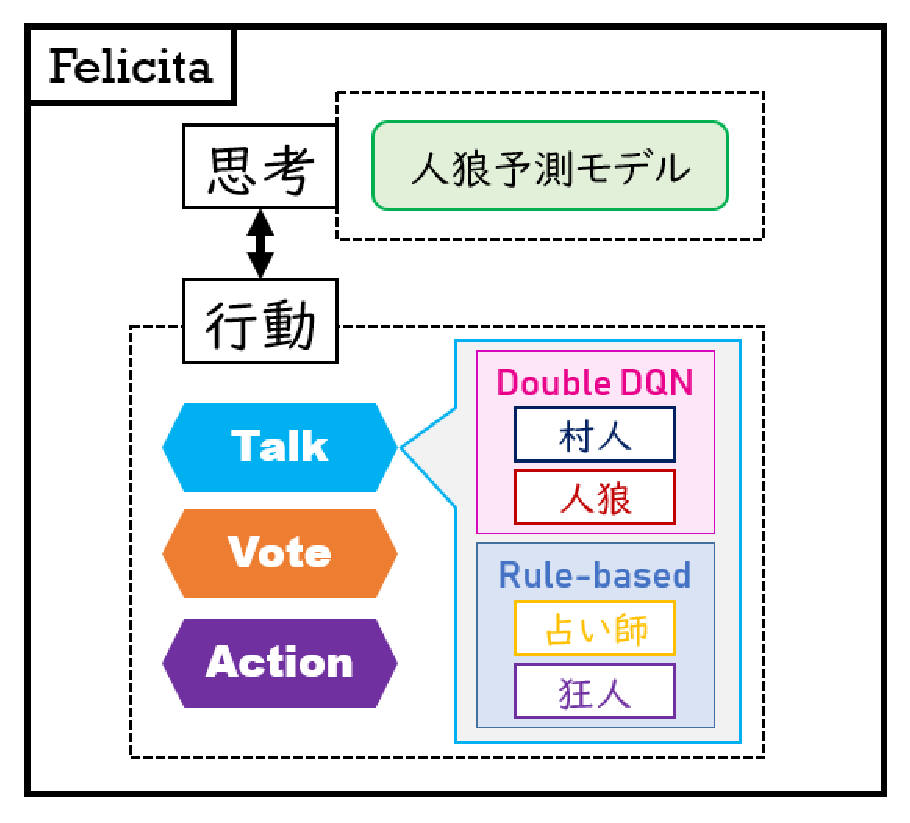
\includegraphics[width = 10cm,clip]{./fig/04.exp/felicita.eps}
      \end{center}
      \caption{エージェント``Felicita'}
     \label{fig:06_fel}
\end{figure}


\begin{table}[t]
		\caption{人狼投票率[\%]}
		\label{tb:06_result1}
		\vspace{3mm}
		\centering
		\begin{tabular}{|c|c|c|c|c|}
			\hline
			\multicolumn{2}{|c|}{}&Felicita&Baseline\_Ave&Baseline\_Best\\
			\hline
			村人&1日目&72.3&59.1&77.1\\
			\cline{2-5}
			&2日目&75.4&68.2&78.1\\
			\hline
			占い師&1日目&75.0&61.1&84.3\\
			\cline{2-5}
			&2日目&87.2&93.1&100\\
			\hline
			狂人&1日目&2.7&15.7&1.3\\
			\cline{2-5}
			&2日目&28.5&30.5&12.8\\
			\hline
		\end{tabular} 
\end{table}





 %数値実験
\clearpage
\newpage
\changeindent{0cm}
\section{まとめと今後の課題}
\label{sec:conclusion}
\changeindent{2cm}

本研究では,
まずDARTSの欠点であるアーキテクチャ構造の制限を緩和するようなネットワーク探索ができた.

また
DARTS に TDGAを組み合わせる提案手法によって,
DARTSのみの結果を超えることができ提案手法の有効性が確認できた.


今後の課題として,
本研究で用いた VGG 以外のネットワークに対してもこの提案手法を適用することで汎用性を確認し,
また他のデータセットや実問題では, 最適なアーキテクチャがどのように変化するか検討することが挙げられる.

(ここに説明を入力)
% ここで 0.5 Page
 %まとめと今後の課題
\clearpage
\newpage
\changeindent{0cm}
\acknowledgements
\changeindent{2cm}


\begin{flushright}
	2021 年 3 月 11 日
\end{flushright}
 %謝辞

\bibliographystyle{./jabbrvunsrt}
% \bibliographystyle{junsrt}
\bibliography{index}
\end{document}
